\documentclass[xcolor={dvipsnames}]{beamer}

\usepackage{beamerthemesplit}
\usepackage{xcolor}
%\startlocaldefs
%\def\argmin{\mathop{\rm arg\,min}\limits}%
%\def\argmax{\mathop{\rm arg\,max}\limits}%
%\endlocaldefs
\usetheme{CambridgeUS}
%\usetheme{Copenhagen}
\usecolortheme{whale}

\definecolor{mycolor}{RGB}{3,86,66}

\setbeamercolor*{structure}{bg=mycolor!20,fg=mycolor}



\setbeamercolor*{palette primary}{use=structure,bg=lightgray,fg=mycolor}
\setbeamercolor*{palette secondary}{use=structure,bg=mycolor,fg=white}
\setbeamercolor*{palette tertiary}{use=structure,bg=black,fg=white}
\setbeamercolor*{palette quaternary}{bg=black,fg=white}
\setbeamercolor*{titlelike}{use=structure,bg=mycolor,fg=white}

\setbeamercolor{frametitle}{bg=structure,fg=white}

%OTHER THEMES: 
% AnnArbor, Antibes, Bergen, Berkeley, Berlin,
% Boadilla, boxes, CambridgeUS, Copenhagen, Darmstadt,
% default, Dresden, Frankfurt, Goettingen, Hannover,
% Ilmenau, JuanLesPins, Luebeck, Madrid, Malmoe,
% Marburg, Montpellier, PaloAlto, Pittsburgh, Rochester,
% Singapore, Szeged, Warsaw

%SEE http://mike.polycat.net/gallery/beamer-themes


%\setbeamercovered{transparent}
\logo{
\includegraphics[height=1.25cm]{1024px-CalPoly_Seal.png}}


%\parskip = .1in
%\usepackage[scale=.75]{geometry}
%\usepackage{amsmath}
\usepackage{graphicx}
\usepackage{amssymb}
\usepackage{epstopdf}
%\usepackage{graphicx}
\usepackage{setspace}
\usepackage{comment}
%\usepackage[dvipdf]{graphicx}

\hypersetup{
    colorlinks=true,
    linkcolor=blue,
    filecolor=magenta,      
    urlcolor=cyan,
}

%
%\setlength{\oddsidemargin}{0.0in}
%\setlength{\topmargin}{-0.5in}
%\setlength{\headheight}{0.20in}
%\setlength{\headsep}{3ex}
%\setlength{\baselineskip}{2ex}
%\setlength{\textheight}{9in}
%\setlength{\textwidth}{6.4in}
%\renewcommand{\baselinestretch}{1.1}

\newcommand{\ft}{\frametitle}
\newcommand{\bi}{\begin{itemize}}
\newcommand{\be}{\begin{enumerate}}
\newcommand{\ei}{\end{itemize}}
\newcommand{\ee}{\end{enumerate}}


\title[]{Using Jupyter to Take Your Data Science Workflow to the Next Level}
\author[Glanz]{Hunter Glanz}
\institute[]{California Polytechnic State University \\ San Luis Obispo, California, USA}
\date{July 24, 2019}

\begin{document}
\frame{\titlepage}


\begin{frame}
\ft{Aims/Themes of This Talk}
\begin{center}
	\emph{Reproducibility} \\
	\pause
	and \\
	\emph{Integration of SAS with open source tools like Jupyter}
\end{center}
\end{frame}

\begin{frame}
\frametitle{Historical Collaboration on Projects}
\bi
	\item Organized, but fragmented...
\ei
\pause
\begin{center}
	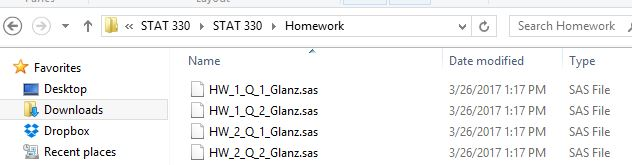
\includegraphics[width = 3in]{STAT330Files.JPG} \\ \vspace{.5in}
	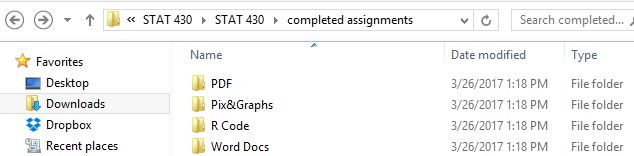
\includegraphics[width = 3in]{STAT331Files.JPG}
\end{center}
\end{frame}

\begin{frame}
\frametitle{Story is Similar between Academia and Industry}
\begin{minipage}{.45\textwidth}
\bi
	\item Clean, wrangle, manage data
	\item Summarize and visualize data
	\item Analyze and model
	\item Synthesize and report
\ei
\begin{center}
	\emph{``Some" assembly required}
\end{center}
\end{minipage}
\begin{minipage}{.45\textwidth}
\begin{center}
	
\includegraphics[width = \textwidth]{flyingpapers.jpg}
\end{center}
\end{minipage}
\end{frame}

\begin{frame}
\ft{Historical Deficiencies}
\begin{minipage}{.45\textwidth}
\begin{center}
	
\includegraphics[width = \textwidth]{hands-putting-puzzle-pieces-together_23-2147513390.jpg}
\end{center}
\end{minipage}
\begin{minipage}{.45\textwidth}
\bi
	\item Fragmented collection of files:
		\bi
			\item Code, text, images, data...
		\ei
	\item Communication, readability, reproducibility suffer
	\item Unnecessarily large distance between data and story
\ei
\end{minipage}
\end{frame}

\begin{frame}
\ft{Does Anything Out There Work?}
\begin{minipage}{.45\textwidth}
\bi
	\item Make computing easier:
		\bi
			\item IDEs and editors (Emacs, Notebook++, Vim, SAS Studio, RStudio, etc.)
		\ei
	\item Make report-writing easier:
		\bi
			\item SAS*, RStudio, LaTeX
		\ei
\ei
\end{minipage}
\begin{minipage}{.45\textwidth}
\begin{center}
	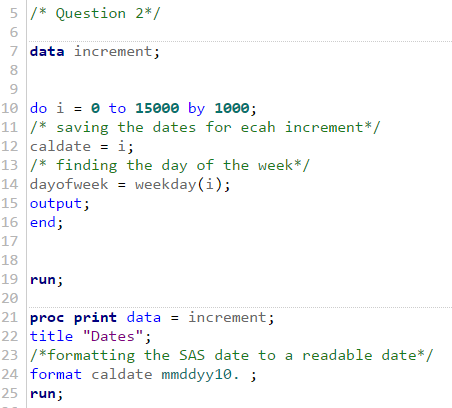
\includegraphics[width = .75\textwidth]{SAS-StudioPic.PNG}
	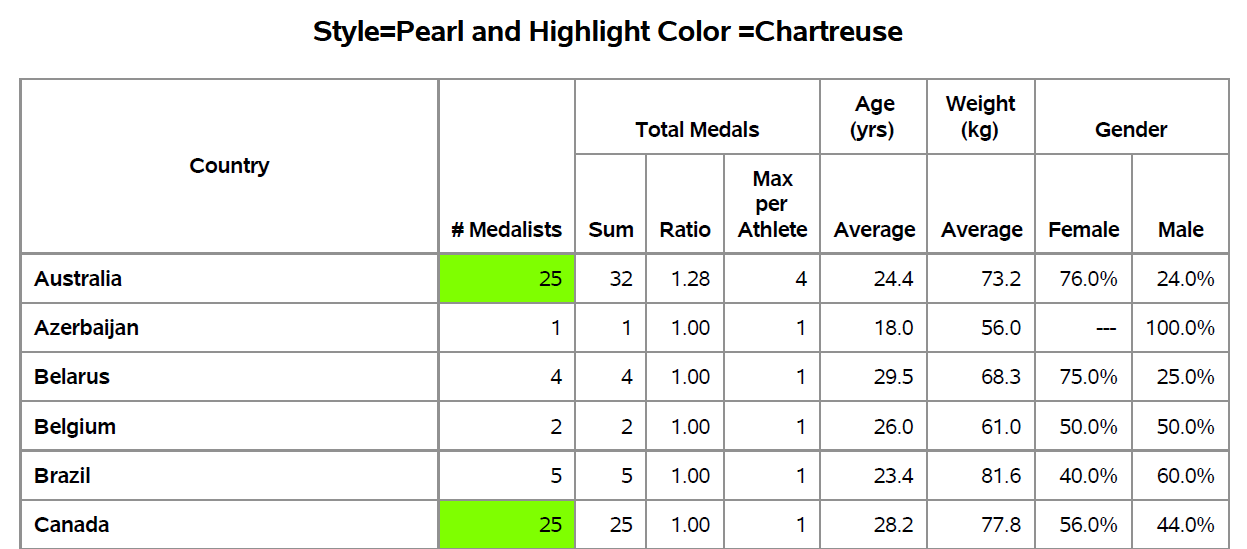
\includegraphics[width = .75\textwidth]{PROC-REPORT-Pic.PNG}
\end{center}
\end{minipage}
\end{frame}


\begin{frame}
\ft{Nothing Addresses Our Needs}
\begin{minipage}{.45\textwidth}
\bi
	\item IDEs/Editors
		\bi
			\item SAS Studio and RStudio
				\bi
					\item Built-in documentation
				\ei
			\item Color coding, formatting, etc.
		\ei
	\item Documenting
		\bi
			\item RMarkdown \& Report-Writing Interface
			\item Highly customizable LaTeX
		\ei
\ei
\begin{center}
	\emph{None of these integrate coding and documentation!}
\end{center}
\end{minipage}
\begin{minipage}{.45\textwidth}
\begin{center}
	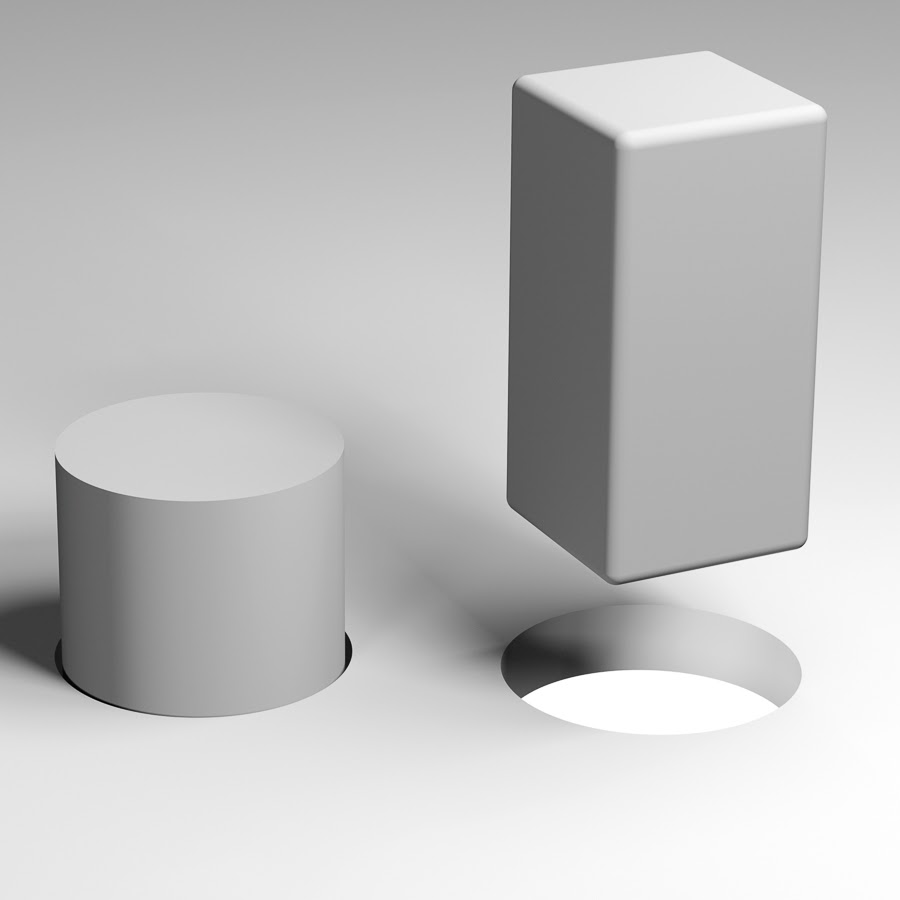
\includegraphics[width = \textwidth]{squarepegroundhole.jpg}
\end{center}
\end{minipage}

\end{frame}


\begin{frame}
\ft{Capabilities of Ideal Tool}
\begin{minipage}{.45\textwidth}
\bi
	\item Color coding, formatting, organization of existing tools
	\item Documentation and report writing organically coexist with coding
	\item Streamline the process of:
		\bi
			\item Exploratory data analysis
			\item Data science
			\item Data journalism
			\item Research
			\item Analytics, etc.
		\ei
\ei
\end{minipage}
\begin{minipage}{.45\textwidth}
\begin{center}
	
\includegraphics[width = \textwidth]{people-gears.PNG}
\end{center}
\end{minipage}
\end{frame}

\begin{frame}
\ft{Cue the Jupyter Project}
\bi
	\item Supports over 40 software languages!
\ei
\begin{center}
	
\includegraphics[width = .5\textwidth]{rectanglelogo-greytext-orangebody-greymoons.png} \\ \vspace{.2in}
	
\includegraphics[width = .5\textwidth]{InUseAt.PNG}
\end{center}
\end{frame}

\begin{frame}
\ft{You May Be....}
\pause
\begin{minipage}{.45\textwidth}
\begin{center}
	
\includegraphics[width = \textwidth]{DistactedJupyterGears.jpg}
\end{center}
\end{minipage}
\pause
\begin{minipage}{.45\textwidth}
\begin{center}
	
\includegraphics[width = \textwidth]{OldWomanComputerMeme.jpg}
\end{center}
\end{minipage}
\end{frame}

\begin{frame}
\ft{Getting Started with Jupyter Notebooks}
\begin{center}
	
\includegraphics[width = .75\textwidth]{SASStudio-JupyterLab.jpg} \\ \vspace{.5in}
	
\includegraphics[width = .75\textwidth]{SASKernel-GitHub-Header.PNG}
\end{center}
\end{frame}

\begin{frame}
\ft{Live Demo of Jupyter via SAS University Edition!}
\begin{center}
	\textbf{\emph{Live Demo!}}
\end{center}
\end{frame}

\begin{frame}
\ft{Project Jupyter Summary Part I}
\bi
	\item Web application enabling creation of documents that contain live code, equations, visualizations and explanatory text.
	\item Over 40 languages are supported, including SAS, Python, and R!
	\item Code within the notebook can produce rich output such as images, videos, LaTeX and JavaScript.
	\item Interactive widgets can be used to manipulate and visualize data in real time.
\ei
\end{frame}

\begin{frame}
\ft{Project Jupyter Summary Part II}
\begin{minipage}{.45\textwidth}
\bi
	\item Nbviewer
	\item GitHub
	\item Binder
	\item JupyterHub (for organizations)
\ei
\end{minipage}
\begin{minipage}{.45\textwidth}
	
\includegraphics[width = \textwidth]{mybinder.png}
\end{minipage}
\end{frame}

\begin{frame}
\ft{Conclusions: Ease of Use}
\bi
	\item From personal use to JupyterHub for organizations, Jupyter Notebooks make statistical computing easier to do AND share than every before!
	
	\begin{center}
		\emph{``The need to minimize \underline{thought-to-execution friction} is probably the single biggest productivity requirement in corporate America."}
	\end{center}
	
	\item Jupyter Notebooks let us take a GIANT leap toward achieving this when it comes to data science and statistical computing.
\ei
\end{frame}

\begin{frame}
\ft{Conclusions: The Tool We Need and Deserve}
\bi
	\item Jupyter Notebooks
		\bi
			\item A single vehicle for live code, text and images.
			\item Dynamic documents that enhance statistical computing and statistical communication.
			\item Streamline the analytics process
				\bi
					\item The color coding, formatting and organization of your favorite editor
					\item Report writing capabilities
					\item The integration and synthesis of these things into a single environment
				\ei
		\ei
\ei
\end{frame}

\begin{frame}
\frametitle{Thank You! Questions?}
\bi
	\item Slides and Live Demo at \href{https://github.com/hglanz/PugSUG2019-GlanzTalk}{https://github.com/hglanz/PugSUG2019-GlanzTalk}
\ei
\end{frame}


\end{document}